Dexterity ellipsoid.

The Jacobian matrix is in the form of:
\begin{eqnarray}
\begin{Bmatrix}
\dot{P_x} \\
\dot{P_y} \\
\dot{P_z} \\
\omega_x \\
\omega_y \\
\omega_z
\end{Bmatrix} &=&
\begin{bmatrix}
J \\
6 \times 2
\end{bmatrix}
\begin{Bmatrix}
\dot{\theta}_1 \\
\dot{\theta}_2
\end{Bmatrix}
\end{eqnarray}

The Jacobian matrix for this problem is:
\begin{eqnarray}
J&=&\begin{Bmatrix}
\vec{a}_0 \times \parens{\vec{P}_E-\vec{P}_{0}} 	&
\vec{a}_1 \times \parens{\vec{P}_E-\vec{P}_{1}} 	\\
\vec{a}_0& \vec{a}_1 \\
\end{Bmatrix}
\end{eqnarray}

Where: 
\input{JacobianParts}

The manipulability of linear velocity is given by $\dot{\vec{x}}=J_{top}\dot{q}$ where $J_{top}$ is square. For the manipulator:
\begin{eqnarray}
J_{top}&=&\begin{bmatrix}
- 20\cdot \sin(\theta_1 + \theta_2) - 20\cdot \sin(\theta_1)&-20\cdot \sin(\theta_1 + \theta_2)\\ 
20\cdot \cos(\theta_1 + \theta_2) + 20\cdot \cos(\theta_1)&20\cdot \cos(\theta_1 + \theta_2)\\ 
\end{bmatrix} \\
B^{-1}&=&(J_{top}J_{top}^T)^{-1} \\ 
B^{-1}_{(1,1)}&=&\begin{bmatrix}
-(\cos(2\cdot \theta_1 + \theta_2) + \cos(2\cdot \theta_1)/2 + \cos(2\cdot \theta_1 + 2\cdot \theta_2) + \cos(\theta_2) + 3/2)/(400\cdot (\cos(\theta_2)^2 - 1))\\ 
\end{bmatrix} \\ 
B^{-1}_{(1,2)}&=&\begin{bmatrix}
(\sin(2\cdot \theta_1 + \theta_2) + \sin(2\cdot \theta_1)/2 + \sin(2\cdot \theta_1 + 2\cdot \theta_2))/(400\cdot \sin(\theta_2)^2)\\ 
\end{bmatrix} \\ 
B^{-1}_{(2,1)}&=&\begin{bmatrix}
(\sin(2\cdot \theta_1 + \theta_2) + \sin(2\cdot \theta_1)/2 + \sin(2\cdot \theta_1 + 2\cdot \theta_2))/(400\cdot \sin(\theta_2)^2)\\ 
\end{bmatrix} \\ 
B^{-1}_{(2,2)}&=&\begin{bmatrix}
(\cos(2\cdot \theta_1 + \theta_2) + \cos(2\cdot \theta_1)/2 + \cos(2\cdot \theta_1 + 2\cdot \theta_2) - \cos(\theta_2) - 3/2)/(400\cdot (\cos(\theta_2)^2 - 1))\\ 
\end{bmatrix} \ 
\end{eqnarray}


The ellipsoid can then be determined from the eigenvalues and eigenvectors of $B^{-1}$ where:

\begin{eqnarray}
a_x&=&\frac{1}{\sqrt{\lambda_1}} \\
b_y&=&\frac{1}{\sqrt{\lambda_2}}  \\
\end{eqnarray}

The rotation through $\beta$ can me found by comparing $B^{-1}$ to the rotation matrix.

\begin{eqnarray}
\theta_1 &=& 264.697437 \\ 
\theta_2 &=& 180.319597 \\ 
a_x &=& 0.111560 \\ 
b_y &=& 20.000000 \\ 
\beta &=& 85.017039 
\end{eqnarray}


\begin{figure}[H]
  \centering
    \includegraphics[height=.6\textwidth]{Ellipsoid1}
 \caption{Ellipsoid immediately after $\omega_1$ reaches its peak}
  \label{Ellipsoid1}
\end{figure}

The ellipsoids approaching $\omega_1$ max (when linkage 1 switches quadrants).
\begin{figure}[H]
  \centering
    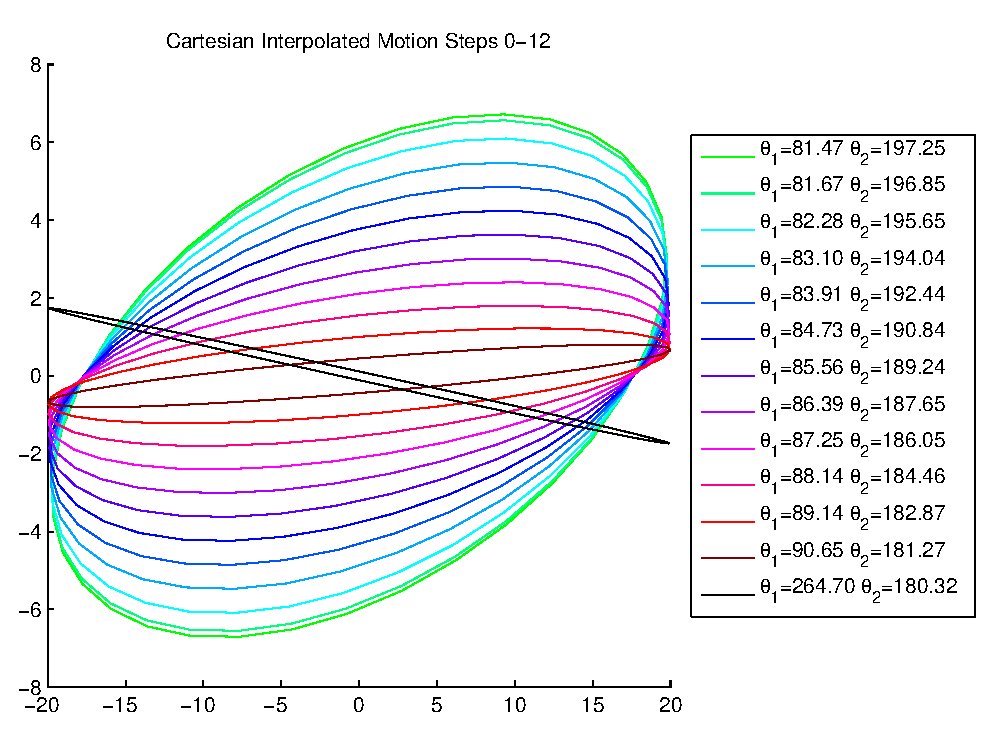
\includegraphics[height=.6\textwidth]{Ellipsoid2}
 \caption{Ellipsoid for points 0-12}
  \label{Ellipsoid2}
\end{figure}